\chapter{Experimental}
\section{Material}

\subsection{Ag(100) crystal}
A \acf{Ag} single crystal from the Diamond Light Source with a crystal orientation of (100) was used as the adsorbent for the \ac{XPS} experiments. It is important that a single crystal is used, as this has a uniform and precisely defined surface and has almost no structural defects.

Silver forms a \ac{fcc} crystal system, which is shown in \autoref{fig:Ag(100)}. This corresponds to the Pearson symbol cF. In the crystal system of silver, one silver atom is surrounded by twelve others. Furthermore, Ag(100) does not reconstruct. The lattice constant of silver in volume is $4.0862\pm0.0002$~\si{\angstrom} at a temperature of $25\pm5$~\si{\celsius}\autocite{Mueller2006,Weast1974}.

\begin{figure}[H]
	\centering
	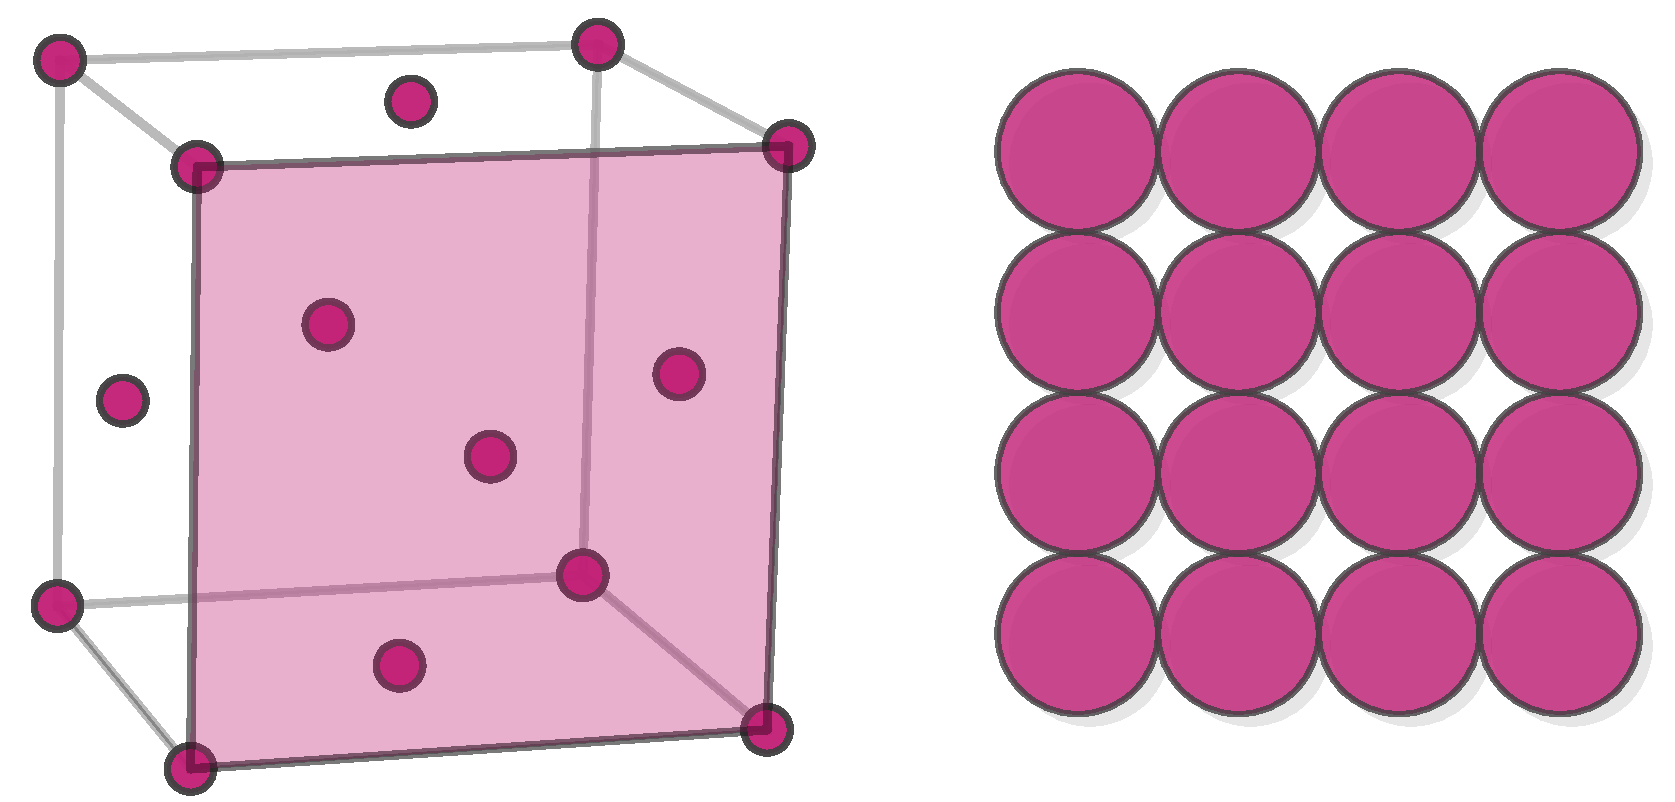
\includegraphics[width=0.9\textwidth]{images/Ag(100).pdf}
	\caption{Unit cell of the silver crystal with marked (100) plane and the surface of Ag(100).}
	\label{fig:Ag(100)}
\end{figure}

As seen in \autoref{fig:Ag(100)}, the surface of the Ag(100) single crystal has a quadratic shape with the lattice constant $4.0862$~\si{\angstrom}/$\sqrt{2}=$2.8894~\si{\angstrom}. The surface has different adsorption sites called fcc, on-top and bridge.

\newpage
\subsection{Quinachridone (QA)}

The examined adsorbate \acf{QA} is a high symmetric, red colored organic molecule with the full IUPAC name 5,12-dihydro-quino[2,3-\textit{b}]acridine-7,14-dione and the sum formula \ce{C20H12N2O2}.
\ac{QA} is most prominently recognized as the parent structure of a group of pigments, most notably Pigment Violet 19 (C.I. 73900). This particular pigment is extensively utilized in industrial applications due to its remerkable color properties and stability.\autocite{ChemBook2025,ChemSpider2025} The molecular structure of \ac{QA} is shown in \autoref{fig:QA}.

\begin{figure}[H]
	\centering
	\begin{subfigure}[b]{0.48\linewidth}
		\centering
		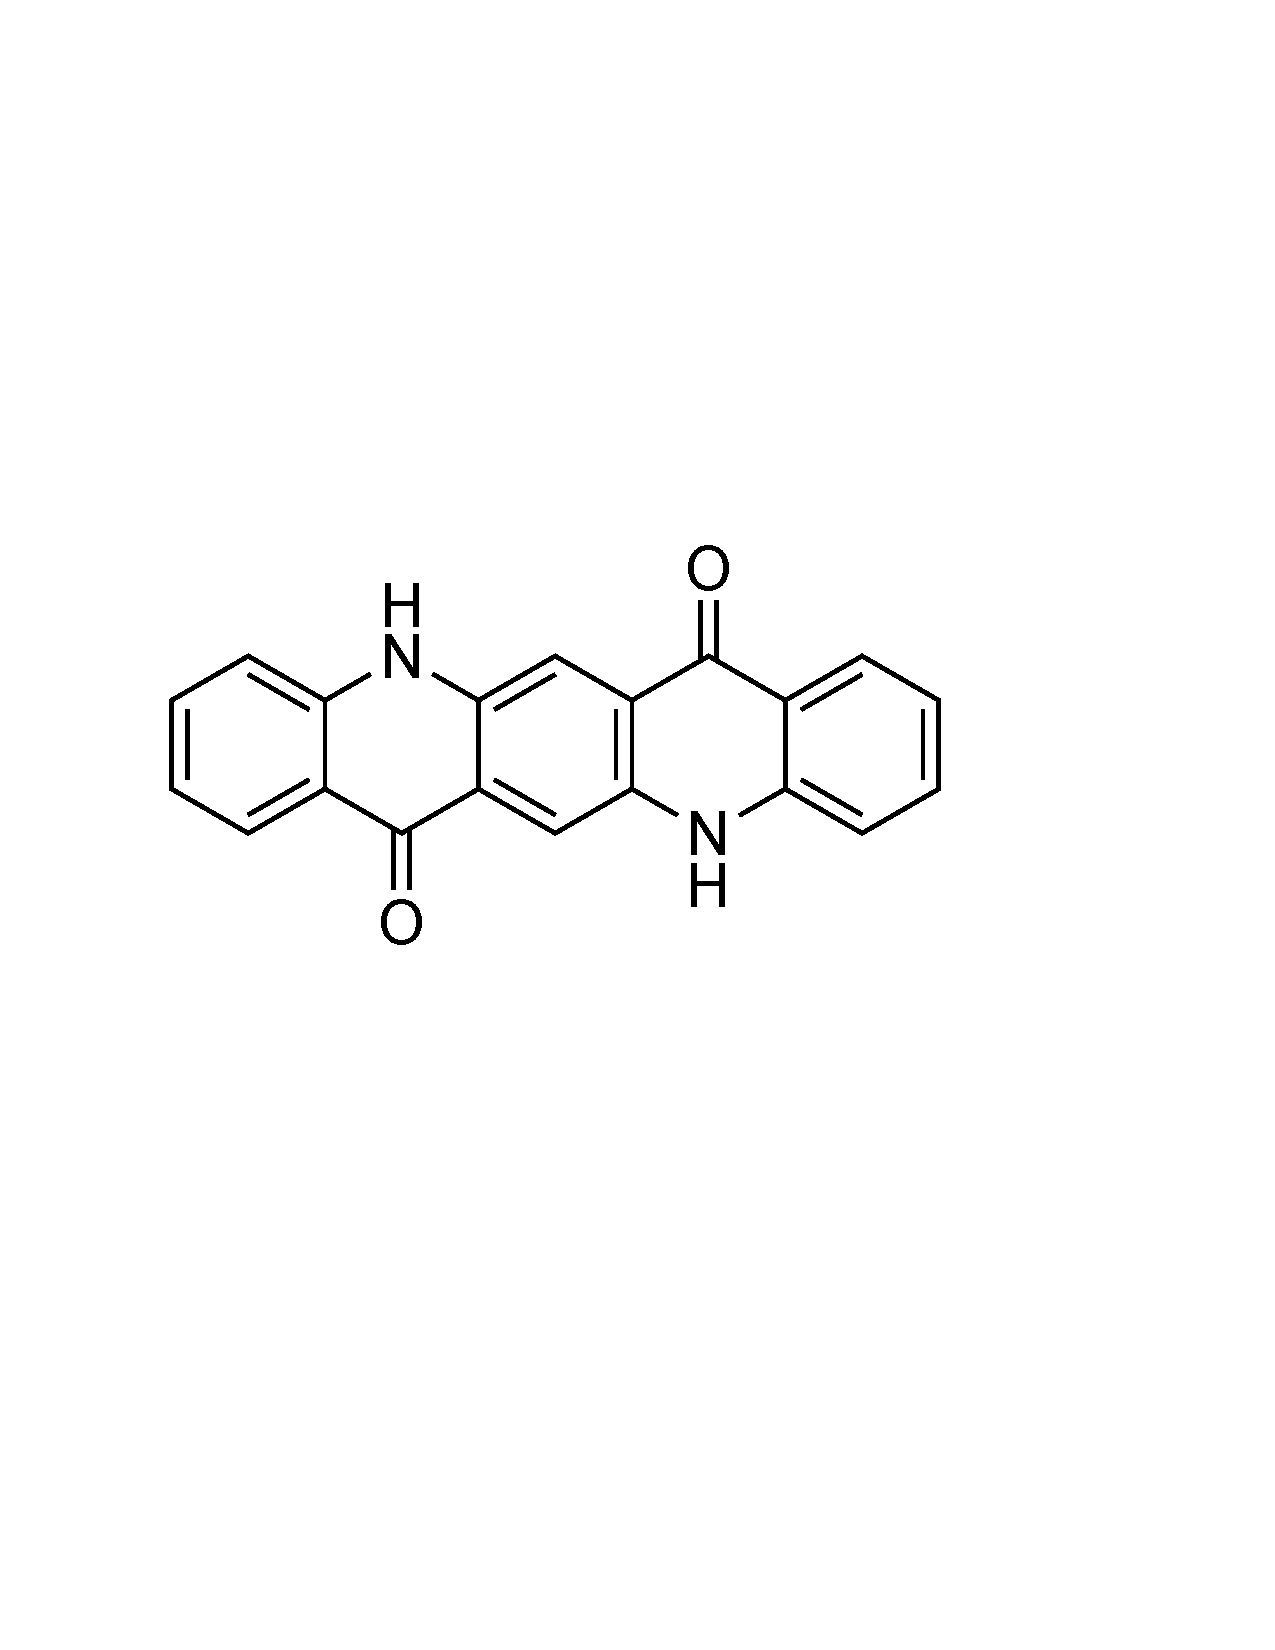
\includegraphics[width=\linewidth]{images/QA.pdf}
		\caption{Skeletal structure}
	\end{subfigure}
	\hfill
	\begin{subfigure}[b]{0.48\linewidth}
		\centering
		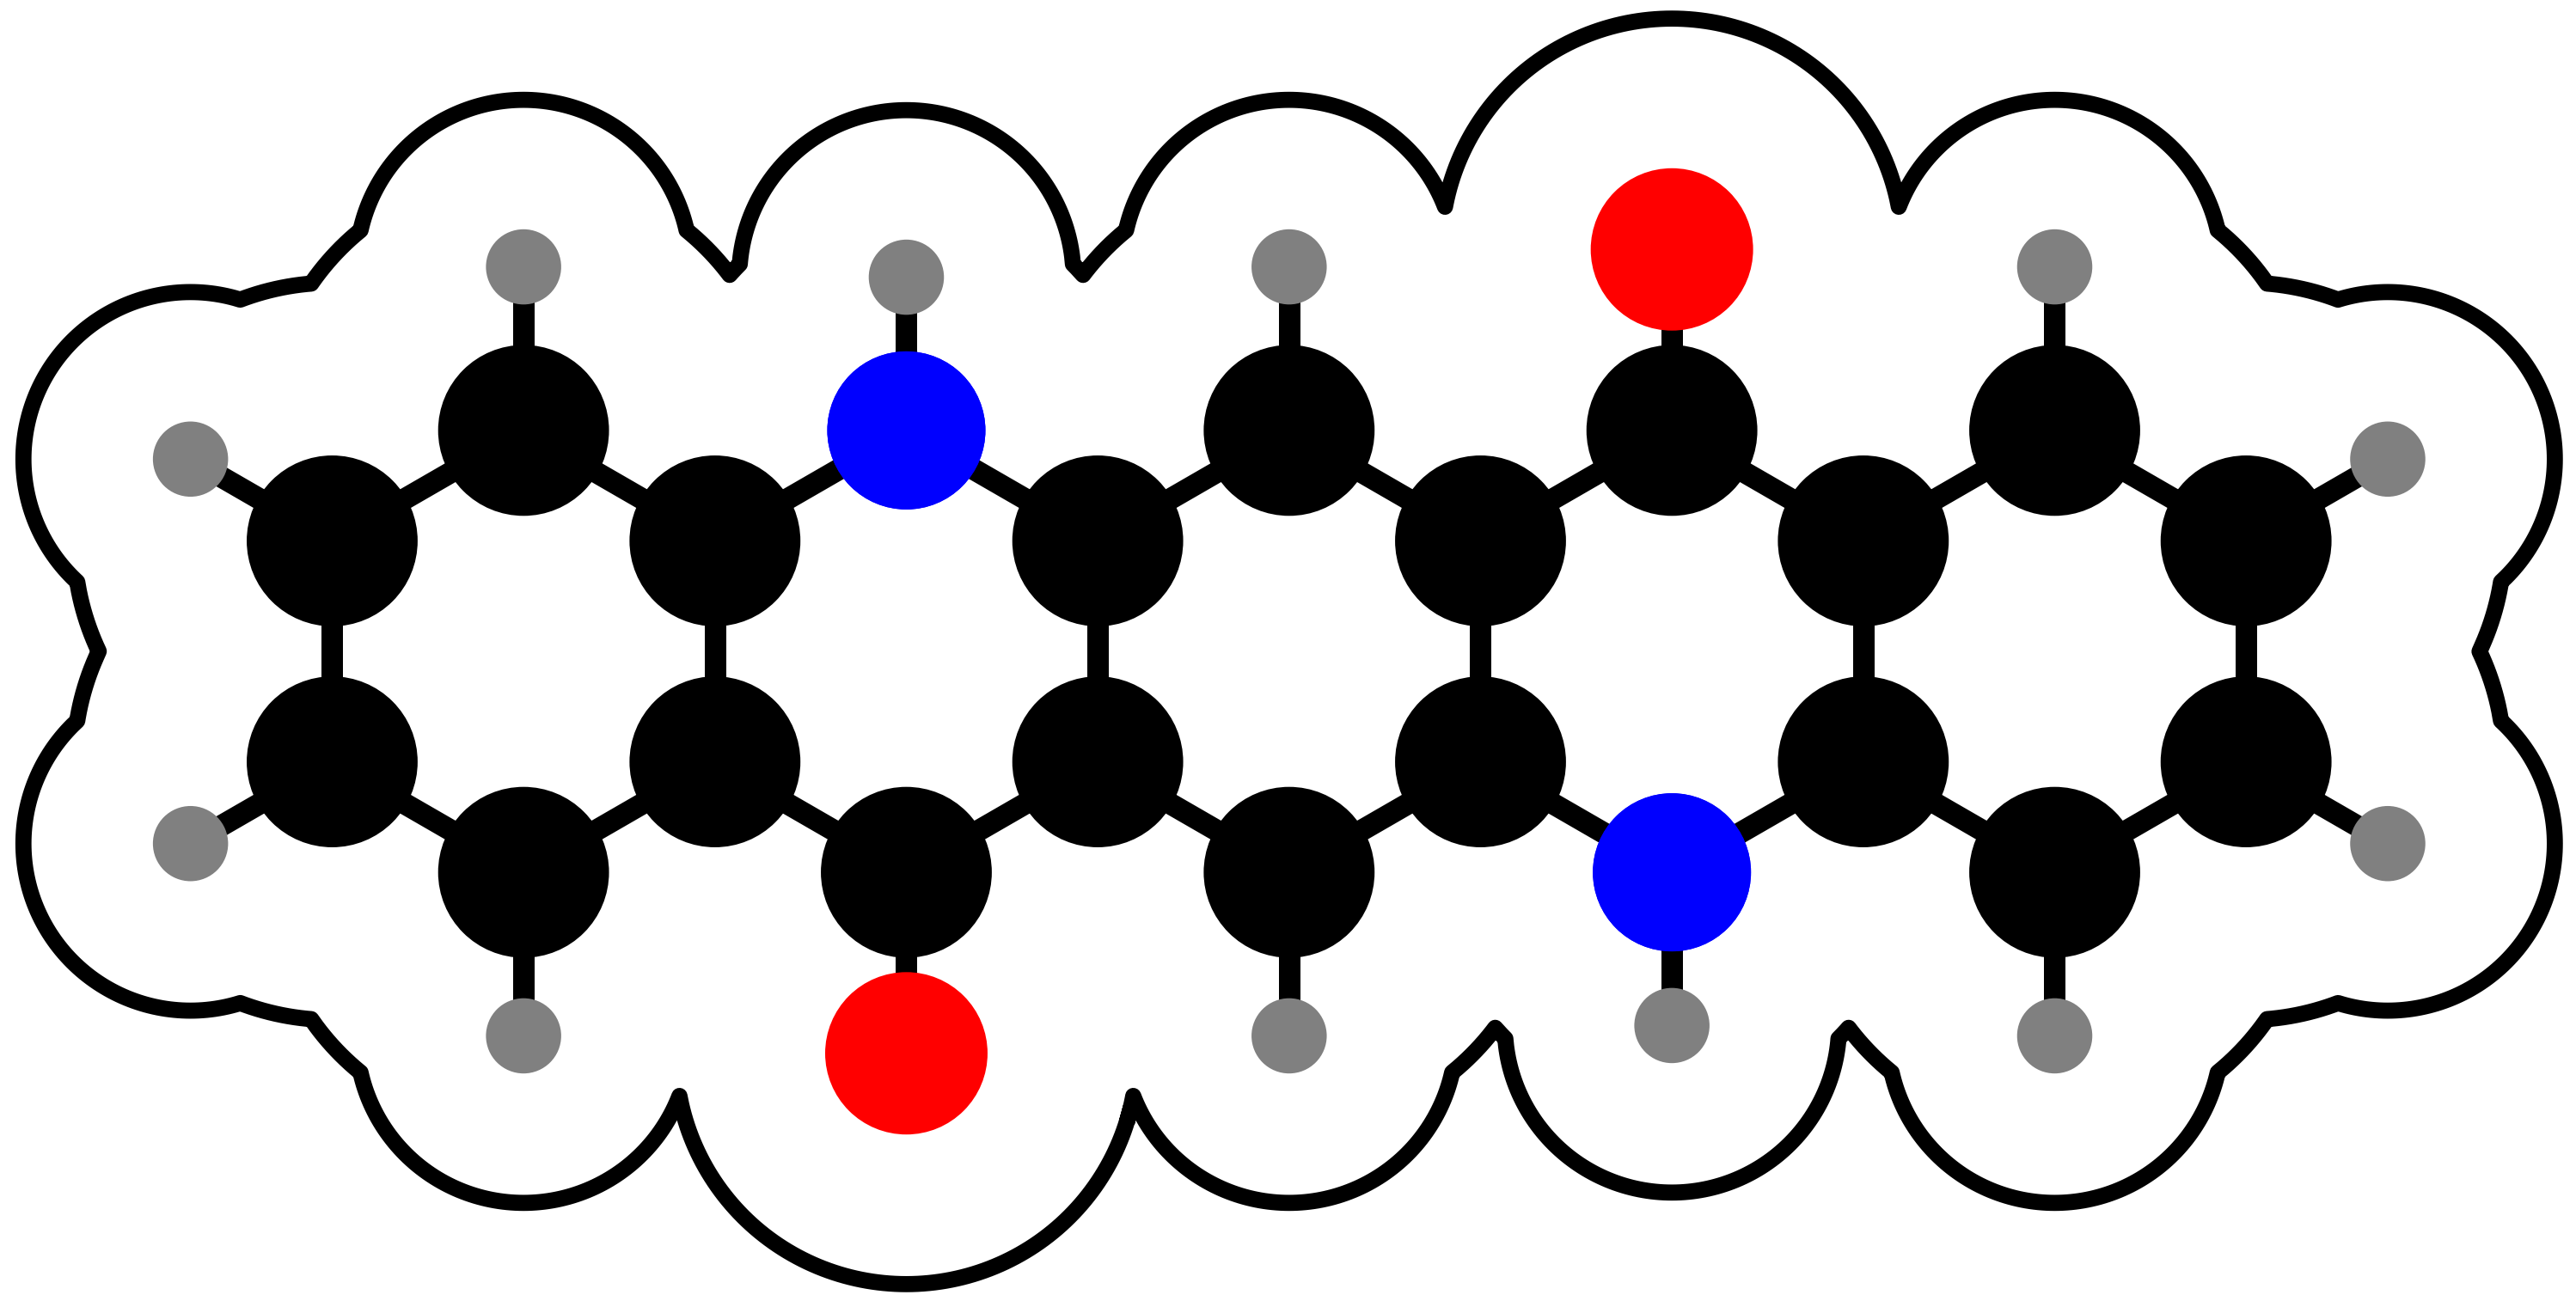
\includegraphics[width=\linewidth]{images/QA_molecule.png}
		\caption{Ball-and-stick model}
	\end{subfigure}
	\caption{Molecular structure of \acf{QA}.}
	\label{fig:QA}
\end{figure}


The molecule is classified as a heterocyclic compound. Its structure is characterized by a conjugated ring system that imparts significant rigidity and planarity to the molecule.\autocite{PubChem2025}. \ac{QA} is of the symmetry group $\mathrm{C_{2h}}$ and has a molar mass of 312.32~\si{g/mol}. The molecule is a crystalline solid with four known different crystal structures under standard conditions.\autocite{Paulus2007,Mizuguchi2002}

\newpage
\section{Experimental setup}

All \ac{XPS} measurements were performed in an \ac{UHV} chamber at the I09 endstation at the Diamond Light Source in Didcot, UK, which is depicted in \autoref{fig:I09}.

\begin{figure}[htbp]
	\centering
	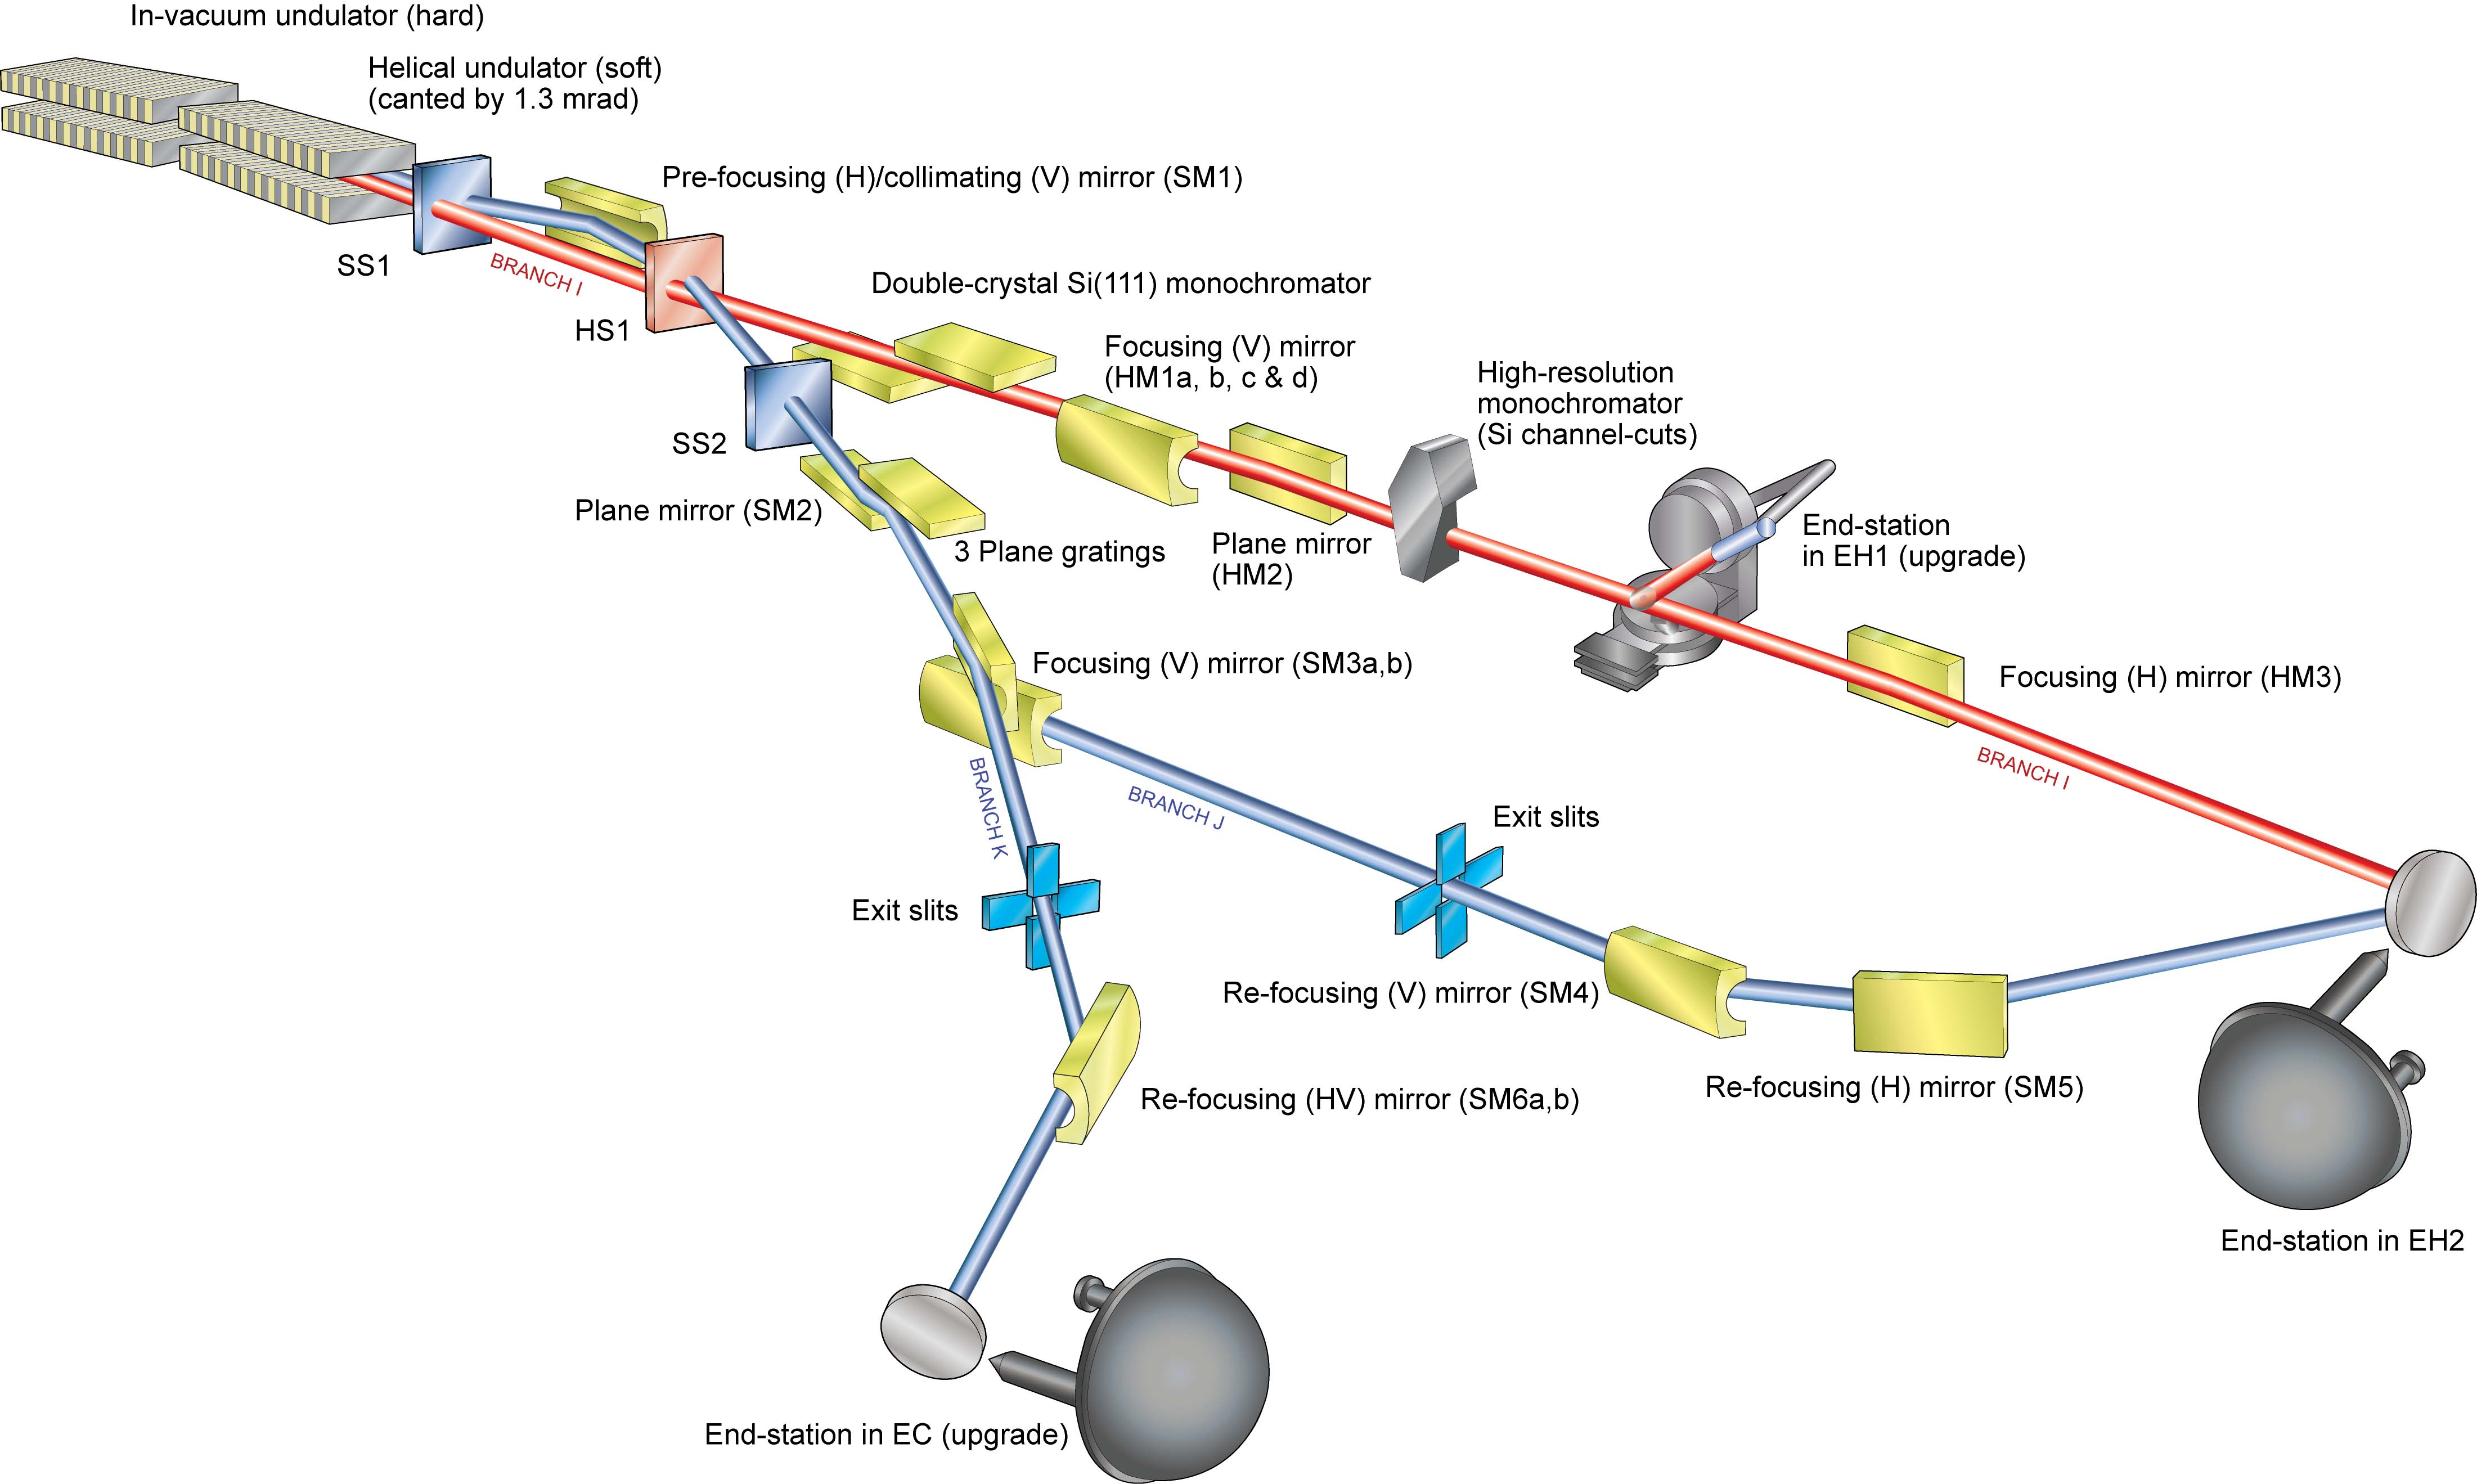
\includegraphics[width=0.9\textwidth]{images/I09.jpg}
	\caption{Schematic drawing of the I09 endstation of the Diamond Light Source in Didcot, UK. Picture taken from \cite{Diamond2025}.}
	\label{fig:I09}
\end{figure}

 This particular endstation utilizes radiation from an undulator located inside the electron storage ring of the synchrotron. The I09 endstation is equipped with a nitrogen-cooled Si(111) double crystal monochromator and a grating monochromator. This setup enables high-intensity and precise x-ray measurements in the soft and hard x-ray ranges. The emitted photoelectrons were detected by a hemispherical EW4000 HAXPES analyzer purchased from Scienta Omicron. The analyzer has an acceptance cone of 56\si{\degree} and was mounted in the photon polarization plane.\autocite{Diamond2025} A schematic drawing of the measurements position is illustrated in \autoref{fig:experimental}.

\begin{figure}[htbp]
	\centering
	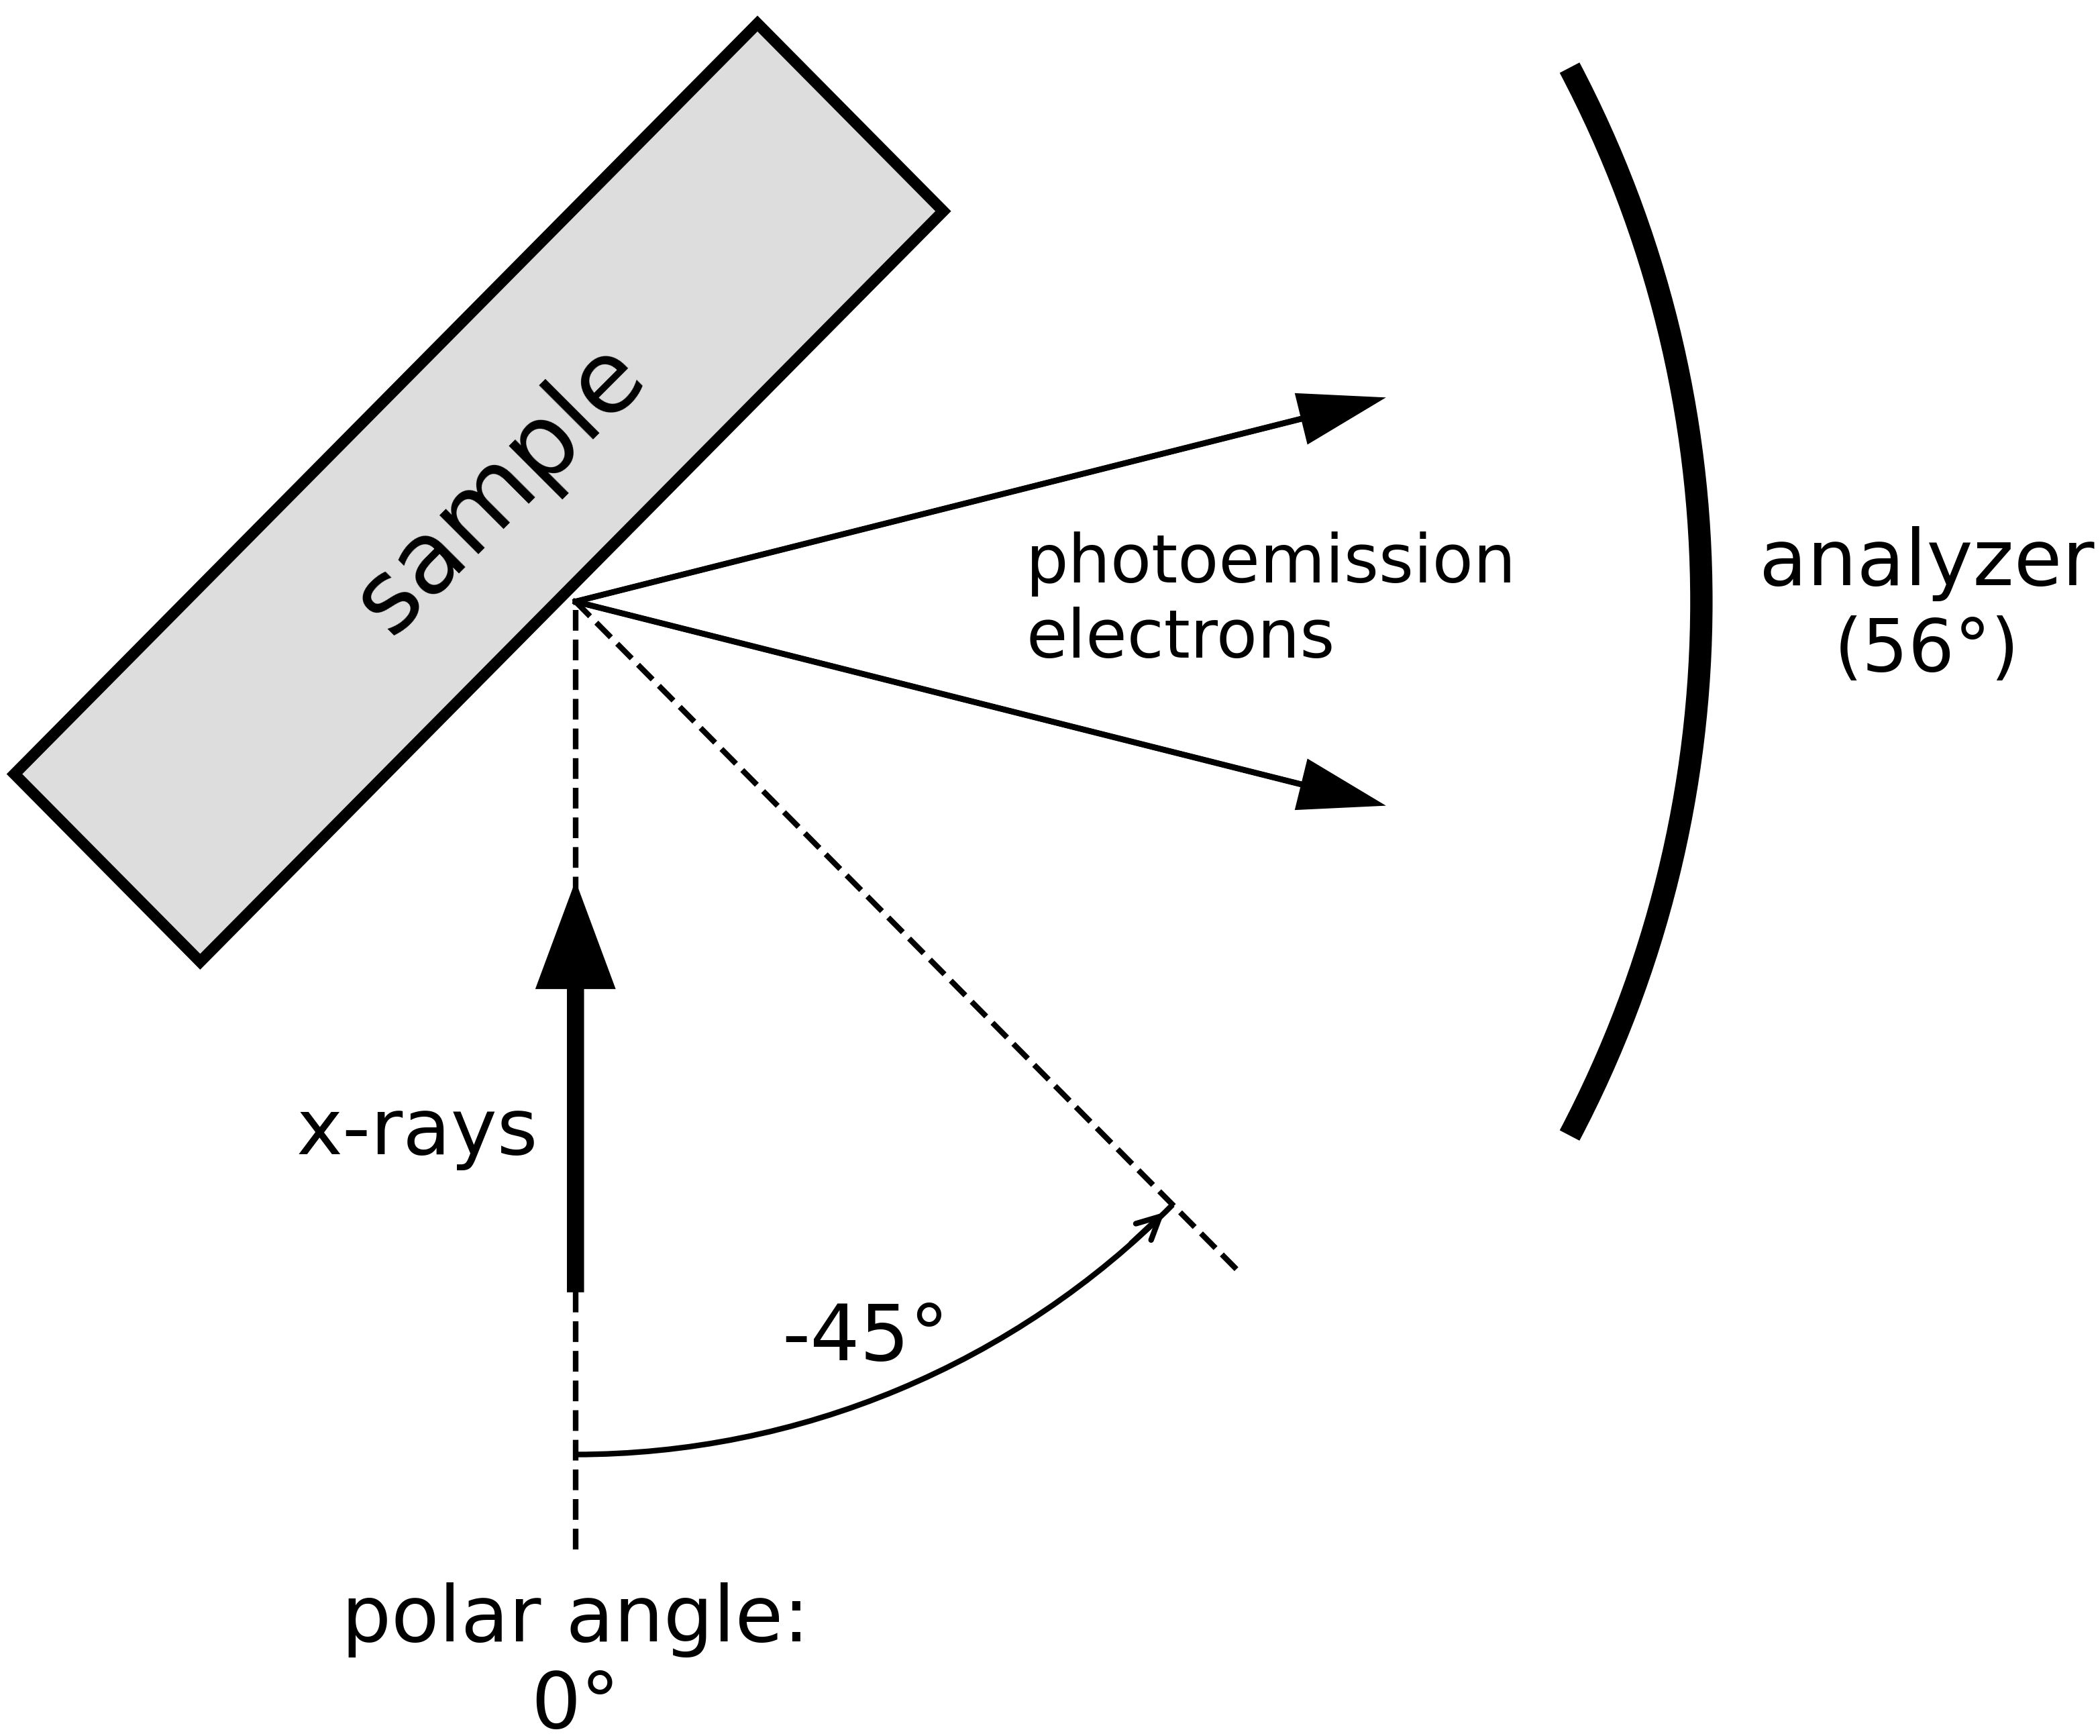
\includegraphics[width=0.6\textwidth]{images/experimental.png}
	\caption{Top view of the sample geometries for the \ac{XPS} measurements at the I09 endstation of the Diamond Light Source in Didcot, UK. Illustrated as in reference \cite{Kny2025}.}
	\label{fig:experimental}
\end{figure}

The experimental preparation for the measurements are described in the following. First, the Ag(100) surface is cleaned by sputtering with argon ions. Therefore, argon is dosed into the chamber up to a pressure of $5\cdot 10^{-5}$~\si{mbar} and is accelerated with a voltage of 1~\si{keV}. Afterwards, the surface is heated up to 825~\si{K} for 45~\si{min} to increase the thermal diffusion and heal defects on the Ag(100) surface.
Subsequently,\ac{QA} was evaporated onto the Ag(100) surface. Therefore, the evaporator was heated to about 500~\si{\degreeCelsius}.

For the measurements of the \ac{XPS} spectra, soft x-ray radiation with an energy of either 500~\si{\eV} for C1s and N1s or 630~\si{\eV} for O1s was used. Therefore, the sample is rotated by -45\si{\degree} in the polar direction toward the analyzer. The detailed parameter for the data acquistion are listed in \autoref{tab:experimental}.

\begin{table}[H]
	\centering
	\caption{Experimental parameter for \ac{XPS} measurements at the I09 endstation of the Diamond Light Sourca in Didcot, UK.}
	\begin{tabular}{|c|c|c|c|c|}
		\hline
		& photon energy $E_\mathrm{\gamma}$ & pass energy $E_\mathrm{pass}$ & step width & number of frames \\
		\hline
		C1s & 500~\si{\eV} & 20~\si{\eV} & 40~\si{meV} & 17 \\
		\hline
		O1s & 630~\si{\eV} & 20~\si{\eV} & 40~\si{meV} & 17 \\
		\hline
		N1s & 500~\si{\eV} & 20~\si{\eV} & 40~\si{meV} & 17 \\
		\hline
	\end{tabular}
	\label{tab:experimental}
\end{table}

\section{Data processing}

The measured data were then subjected to an initial processing stage, whereby the values from multiple datasets employing identical settings for the measurements were averaged. Subsequently, the data underwent further processing with the software CasaXPS.\autocite{CASA2022} Each XPS spectrum was processed in a consistent manner, as outlined below.

Initially, the \ac{BE} of the \ac{XPS} spectrum was calibrated against the Fermi energy $E_\mathrm{F}$. Small inaccuracies of all measurement devices may lead to inaccuracies in the \ac{BE}. Therefore, a \ac{XPS} spectrum of the Fermi edge with same photon energy as the corresponding component \ac{XPS} spectrum is used and fitted with a Fermi function. Without inaccuracies of the devices, $E_\mathrm{F}$ should be zero and for this reason the obtained Fermi energy is then used for the \ac{XPS} spectrum of the component to calibrate the \ac{BE}.

Afterwards, a linear background was fitted to the raw and averaged data. This background is then substracted for further data processing. Afterwards, the corresponding fitting models from \autoref{sec:results} were applied. Therefore, the different peaks with line shape and constraints from \autoref{tab:casa} were used. These settings are the same for each processed dataset.
Subsequently, the processed data was then exported from CasaXPS and illustrated using a customized python script, enabling the generation of various plots as outlined in \autoref{sec:results}.


\begin{table}[H]
	\centering
	\caption{Used parameter in CasaXPS\autocite{CASA2022} for the different peaks of the \ac{XPS} spectra of \ac{QA} on Ag(100) at the I09 endstation of the Diamond Light Sourca in Didcot, UK.}
\begin{tabular}{|c|c|c|}
	\hline
	~~~~~~peak~~~~~~ & ~~~~~~line shape~~~~~~ & ~~~~~~area constraint~~~~~~ \\
	\hline
	$\mathrm{C_{arom}}$ & LA(1,8,800) & 10 \\
	\hline
	$\mathrm{C_{NH}}$ & LA(1,8,800) & 4 \\
	\hline
	$\mathrm{C_{CO}}$ & LA(1,8,800) & 4 \\
	\hline
	$\mathrm{C_{O}}$ & LA(1,8,200) & 2 \\
	\hline \hline
	O1 & LA(1,8,400) & 1 (for $\beta$-phase) \\
	\hline
	$\mathrm{O1_{sat}}$ & LA(1,1,400) &  \\
	\hline
	O2 & LA(1,8,400) & 1 (for $\beta$-phase) \\
	\hline
	$\mathrm{O2_{sat}}$  & LA(1,1,400) &  \\
	\hline \hline
	N1 & LA(1,8,400) & 1 (for $\beta$-phase) \\
	\hline
	$\mathrm{N1_{damage}}$  & LA(1,8,400) &  \\
	\hline
	N2 & LA(1,8,400) & 1 (for $\beta$-phase) \\
	\hline
\end{tabular}
	\label{tab:casa}
\end{table}

\cleardoublepage
